%! Author = mkeim
%! Date = 7/18/24

\section{RP2. Diachronic Word Embeddings Reveal Statistical Laws of Semantic Change} \label{sec:paper_hamilton}
\subsection{Introduction}\label{subsec:hamilton_introduction}
Hamilton et al.\ (2016) explores the dynamic nature of language by analyzing how word meanings evolve over time.
Using \emph{diachronic} (historical) word embeddings, a technique that maps words into vector spaces based on historical corpora, the study uncovers patterns and laws governing semantic shifts.
Their approach provides a quantitative framework to examine how words change meaning, influenced by cultural, and linguistic factors.

The pace at which words undergo semantic change differs, with some words changing meaning more frequently compared to others.
For example, the word `cat' has remained relatively stable in its meaning, while `cast' has evolved to have multiple meanings ~\cite{hamilton-etal-2016-diachronic}.

There are several hypotheses about the patterns in semantic change, including the increasing subjectification of meaning or the grammaticalization.
This paper, however, focuses on following two specific questions about semantic change:
\begin{itemize}
    \item \para{RQ1.} \emph{What role does word frequency play in the evolution of word meanings?}\\
    Frequency is a significant factor in linguistic changes, with high-frequency words often changing faster, while low-frequency words tend to be more resistant to change.
    The connection between word frequency and semantic change is a key unanswered question in the field of linguistics.
    The authors introduce the \textbf{law of conformity} to address this gap, demonstrating that frequent words change more slowly, and it clarifies the role of frequency in semantic change.

    \item \para{RQ2.} \emph{How does polysemy relate to semantic change?}\\
    Another unresolved question in linguistics is the relationship between semantic change and polysemy.
    Polysemous words, which have multiple meanings, appear in a variety of contexts.
    It remains unclear whether the diverse contextual use of these words makes them more or less prone to undergoing semantic change.
    The authors propose the \textbf{law of innovation}, which demonstrates that polysemous words are more likely to experience faster semantic changes.
    If a word has multiple meanings, it is more likely to lead to semantic change, especially in the case of rare senses.
\end{itemize}

In our work on data voids, we have recognized that word frequency significantly impacts their identification.
For instance, the term `sandy' saw a spike in usage during the Hurricane Sandy event (\Cref{subsec:kulkarni-results}).
Similarly, terms associated with political agendas also experience increased usage during relevant events.
This paper provides insights into how frequency influences the evolution of word meanings.

Additionally, our study identifies data voids involving polysemous terms, such as `migrant caravan.'
This term began to change in meaning when FOX News used it to describe people moving from the Mexico border towards the US, and it continued to evolve with new groups of migrants.
Understanding these kinds of data voids is crucial, and this paper helps us identify subtle semantic changes in words with multiple meanings,
enhancing our understanding of how these changes relate to frequency and context.

The paper aims to develop a robust methodology for quantifying semantic change using word embeddings and comparing different approaches to analyzing semantic change.
This methodology is then applied in a large-scale cross-linguistic analysis spanning 200 years and four languages
(English, German, French, and Chinese) to propose the above two statistical laws relating frequency and polysemy to semantic change.

\subsection{Constructing Word Embeddings.}\label{subsec:constructing-word-embeddings}
The authors employ three methods to construct word embeddings for different time periods.
Initially, they create embeddings for each distinct period and then align these embeddings over time to maintain consistency.
To quantify semantic change, they use various metrics.
Specifically, they utilize Singular Value Decomposition (SVD), Positive Pointwise Mutual Information (PPMI), and Skip-Gram with Negative Sampling (SGNS).
These distributional techniques represent each word by a vector that encapsulates information about the word’s co-occurrence statistics.

\para{Positive Pointwise Mutual Information (PPMI). }
PPMI is a statistical measure used to quantify the association between a word and its context within a corpus.
In the paper, it is used to create word embeddings by capturing the strength of association between words and their co-occurring contexts over time.

First, a co-occurrence matrix is built, where each entry represents the frequency with which a word (target) and its context (typically a window of neighboring words) appear together in the corpus.
The \emph{joint probability} of a target word $w_i$ and a context word $c_j$ is calculated by dividing the co-occurrence frequency of $w_i$ and $c_j$ by the total number of word pairs in the corpus.
The \emph{marginal probability} of the target word $w_i$ and the context word $c_j$ are calculated based on the total occurrences of each word in the corpus.
The Positive Pointwise Mutual Information (PPMI) between the target word $w_i$ and the context word $c_j$ is calculated using the formula:
\begin{equation}
\mathbf{M}^{\text{PPMI}}_{i,j} = \max \left\{ \log \left( \frac{\hat{p}(w_i, c_j)}{\hat{p}(w_i) \hat{p}(c_j)} \right) - \alpha, 0 \right\},
\label{eq:ppmi}
\end{equation}

where:
\begin{itemize}
\item $\hat{p}(w_i, c_j)$ is the \emph{joint probability} of the target word $w_i$ and the context word $c_j$ occurring together.
\item $\hat{p}(w_i)$ and $\hat{p}(c_j)$ are the \emph{marginal probabilities} of the target word $w_i$ and the context word $c_j$, respectively.
\item $\alpha > 0$ is a positive constant used to smooth the values and prevent extreme positive values in the PPMI calculation.
\end{itemize}

This formula refines the PPMI measure by incorporating $\alpha$ to adjust the log probability ratio.
The inclusion of $\alpha$ helps manage the sparseness of the data and the impact of low-frequency events, making the measure more robust and stable.

\para{Singular Value Decomposition (SVD). }
SVD is a mathematical technique that factorizes a matrix into three other matrices, revealing important features of the original matrix.
In the context of word embeddings, SVD helps to reduce the dimensionality of the data while preserving the essential structure and patterns in word co-occurrences.
SVD decomposes the co-occurrence matrix into three matrices in the following manner:
\begin{equation}
\mathbf{w}_i^{\text{SVD}} = (\mathbf{U} \Sigma^\gamma)_i,
\label{eq:svd}
\end{equation}

where:
\begin{itemize}
    \item $\mathbf{w}_i^{\text{SVD}}$ is the vector representation of the word $w_i$ in the SVD-based embedding space.
    \item $\mathbf{U}$ is the matrix of left singular vectors obtained from the decomposition of the co-occurrence matrix.
    \item $\Sigma$ is the diagonal matrix of singular values.
    \item $\gamma$ is a parameter that scales the singular values, allowing for tuning the influence of the different components.
\end{itemize}

In this formula, the word vector $\mathbf{w}_i^{\text{SVD}}$ is derived by scaling the singular values in $\Sigma$ by $\gamma$ and then multiplying by the corresponding vectors in $\mathbf{U}$.
This approach provides a flexible way to adjust the contribution of the components to the final word embeddings.

\para{Skip-Gram with Negative Sampling (SGNS). }
SGNS is a technique used to learn high-quality word vectors by training on large corpora.
The primary goal of SGNS is to learn word embeddings such that words that appear in similar contexts have similar vector representations.
For a given target word $w$ and a context word $c$, the model tries to maximize the probability $P(c|w)$
\begin{equation}
\hat{p}(c_i \mid w_i) \propto \exp(\mathbf{w}_i^{\text{SGNS}} \cdot \mathbf{c}_j^{\text{SGNS}}),
\label{eq:sgns}
\end{equation}

where:
\begin{itemize}
    \item $\hat{p}(c_i \mid w_i)$ is the estimated probability of a context word $c_i$ given a target word $w_i$.
    \item $\mathbf{w}_i^{\text{SGNS}}$ is the vector representation of the target word $w_i$ in the SGNS embedding space.
    \item $\mathbf{c}_j^{\text{SGNS}}$ is the vector representation of the context word $c_j$ in the SGNS embedding space.
\end{itemize}

The probability $\hat{p}(c_i \mid w_i)$ that a word $c_i$ is a context word of $w_i$ is proportional to the exponential of the dot product of their corresponding vector representations.
The dot product $\mathbf{w}_i^{\text{SGNS}} \cdot \mathbf{c}_j^{\text{SGNS}}$ measures the similarity between the target word and the context word in the vector space.
A higher dot product indicates that the words are more likely to co-occur, leading to a higher estimated probability.

The model uses this probability estimation to distinguish true word-context pairs from randomly sampled negative pairs.
The training objective is to maximize the probability of observed (target, context) pairs and minimize the probability of randomly sampled pairs, thereby learning embeddings that reflect the semantic relationships between words.

\para{Aligning Embeddings.}
Words that have similar meanings across different time periods should ideally have similar embeddings.
Alignment ensures that the embeddings from different periods are comparable, making it possible to observe how a word’s meaning shifts over time.

This alignment process involves finding the best way to rotate and transform the embeddings from one time period so that they closely match the embeddings from the next period.
This is done by finding an orthogonal transformation matrix (let’s call it $\mathbf{R}^{(t)}$) that minimizes the difference between the embeddings from two consecutive time periods.
The transformation ensures that distances and angles between word vectors (which represent their meanings) are preserved, allowing for an accurate comparison.
By aligning the embeddings, the authors could measure the semantic displacement of words—how much the meaning of a word has shifted from one time period to another.

\subsection{Takeaways}\label{subsec:hamilton_takeaways1}
The authors created three types of word embeddings using PPMI, SVD, and SGNS, each capturing different information.
PPMI measures how closely related two words are, resulting in sparse, high-dimensional vectors.
SVD simplifies this information by reducing the dimensionality of the PPMI matrix into dense, low-dimensional vectors.
Lastly, SGNS learns embeddings by predicting surrounding words in a given context, uncovering deeper semantic and contextual nuances that the other methods may not capture.
Additionally, they employed alignment technique to align word embeddings across different time periods, ensuring consistency and enabling the analysis of semantic shifts over time.

\subsection{Measuring Semantic Change}\label{subsec:measuring-semantic-change}
Once the embeddings are aligned, following methods are performed to quantify how much the meaning of word changes over time.
\begin{itemize}
    \item \para{Pair-wise similarity time-series}
        This method measures changes in the similarity between pairs of words over different time periods using cosine similarity.
        \begin{equation}
            s^{(t)}(w_i, w_j) = \text{cos-sim}(w_i^{(t)}, w_j^{(t)})
            \label{eq:equation2}
        \end{equation}
        The Spearman correlation $(\rho)$ is employed to measure the relationship between the similarity scores of word pairs and time.
        This non-parametric method assesses whether the similarity series shows a significant increase or decrease over time, which helps us identify specific linguistic or cultural shifts.

    \item \para{Measuring semantic displacement}
        This method quantifies how much a word's meaning has changed by calculating the displacement of its vector representation across different time points.
        They use the aligned word vectors to compute the \emph{semantic displacement} that a word has undergone during a certain time-period.
        It is measured by calculating the distance between the vector representations of a word in different time periods.
        For a given word $w$, if $\mathbf{w}^{(t1)}$ and $\mathbf{w}^{(t2)}$ are its embeddings in two time periods $t1$ and $t2$, respectively, then the semantic displacement $\Delta$ is computed as:
        \begin{equation}
            \Delta(w) = \text{cos-dist}(\mathbf{w}^{(t1)}, \mathbf{w}^{(t2)}).\label{eq:equation3}
        \end{equation}
\end{itemize}

\subsection{Evaluation \& Results}\label{subsec:evaluation&results}
In this paper, the authors compared different word embedding approaches — PPMI, SVD, and SGNS \Cref{subsec:constructing-word-embeddings} by evaluating them
on \emph{synchronic accuracy} (similarity within time-period) and \emph{diachronic validity} (semantic changes over time).

%\begin{figure}[htb]
%    \centering
%    \vspace{-1em}
%    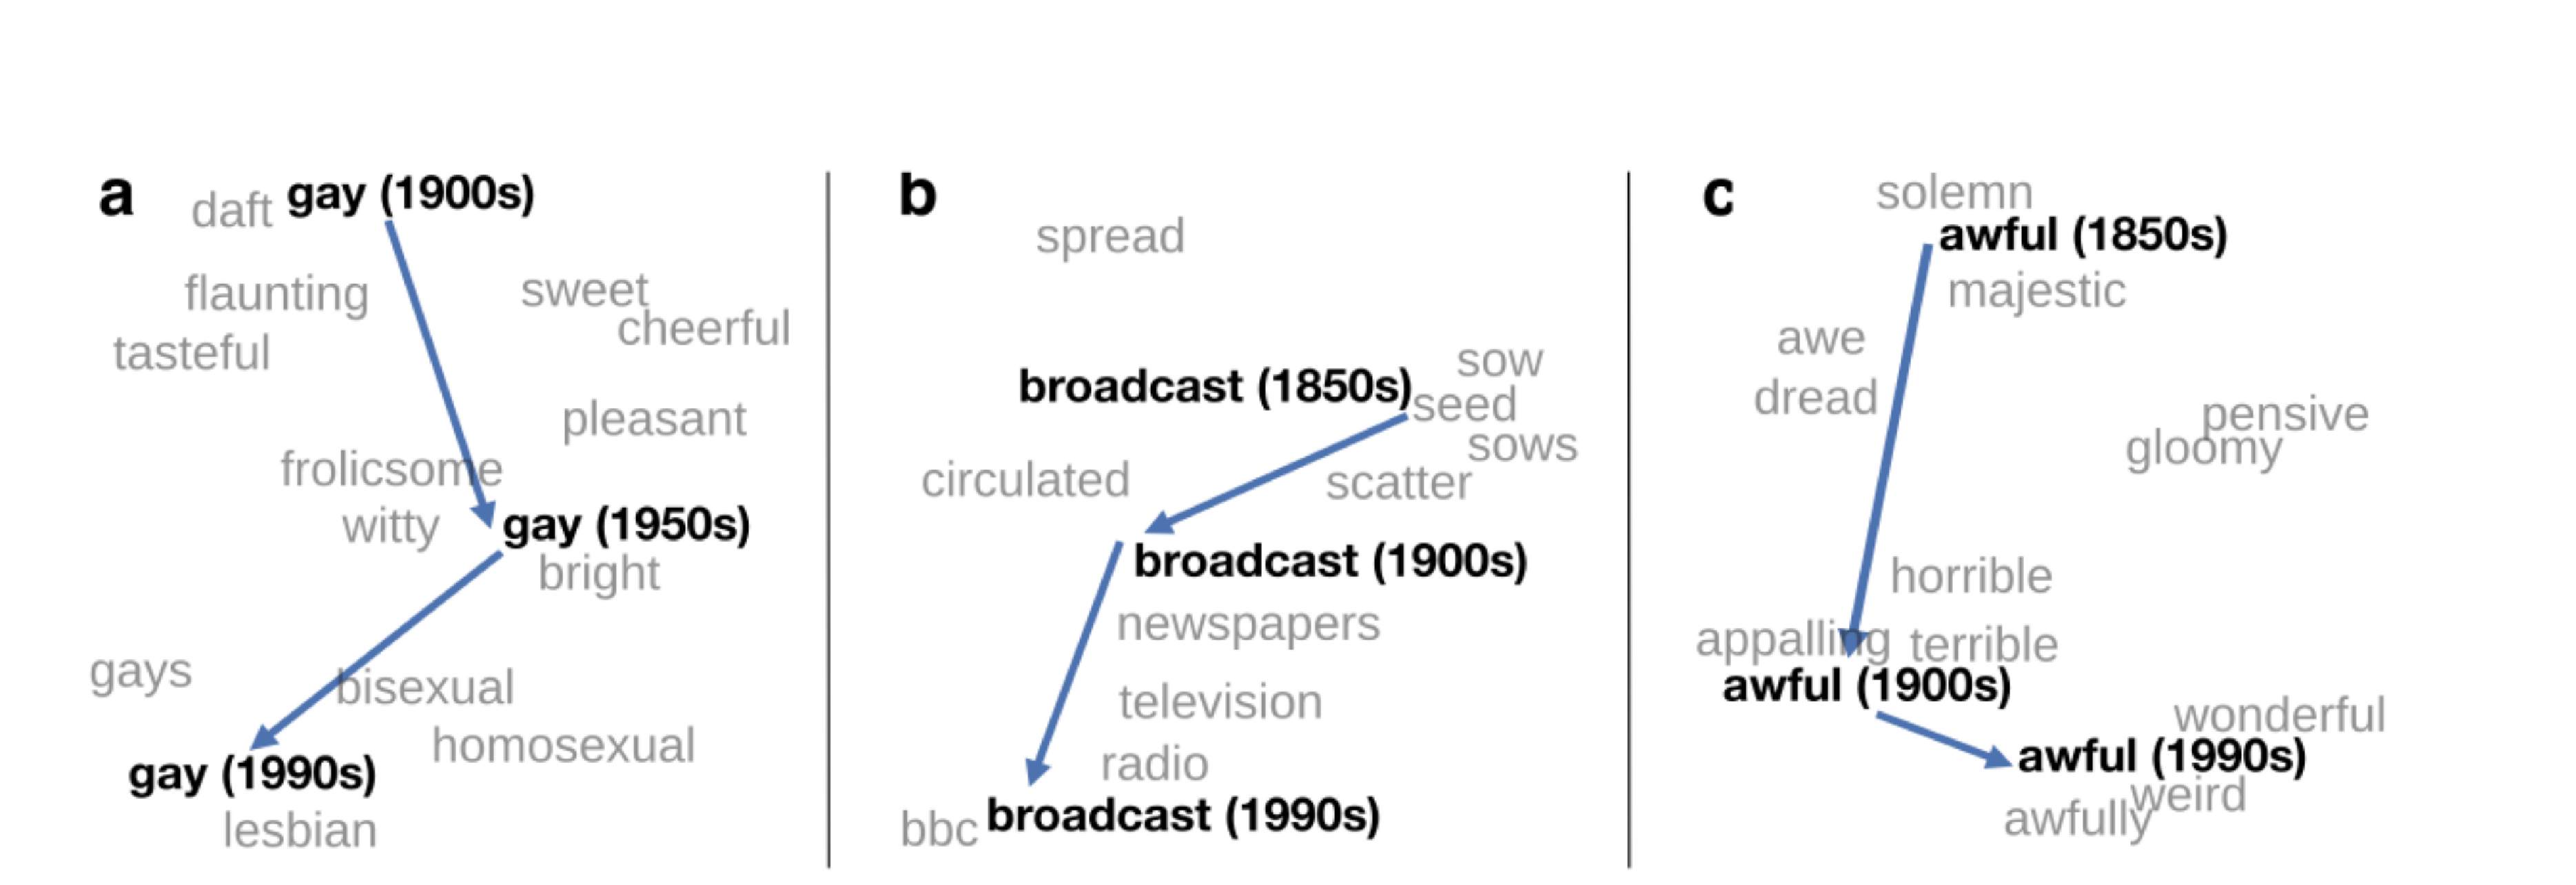
\includegraphics[scale=0.17]{figures/hamilton}
%    \vspace*{-0.5cm}
%    \caption{Example of word 'gay' undergoing change in meaning over time (taken from \cite{hamilton-etal-2016-diachronic}).}
%    \label{fig:hamilton-example}
%\end{figure}

\para{Synchronic Accuracy.}
Synchronic accuracy refers to the accuracy with which word embeddings capture the semantic relationships and meanings of words at a \emph{specific point in time}.
It assesses how well the models represent the semantic relationships among words in a given time period.
SVD performed best here followed by PPMI and SGNS\@.

\para{Diachronic Validity.}
Diachronic validity evaluates how effectively the methods can detect and quantify changes in \emph{meaning over time}.
The authors evaluate the diachronic validity of their methods through two main tasks:

\begin{figure}[tbh]
    \centering
    \vspace{-1em}
    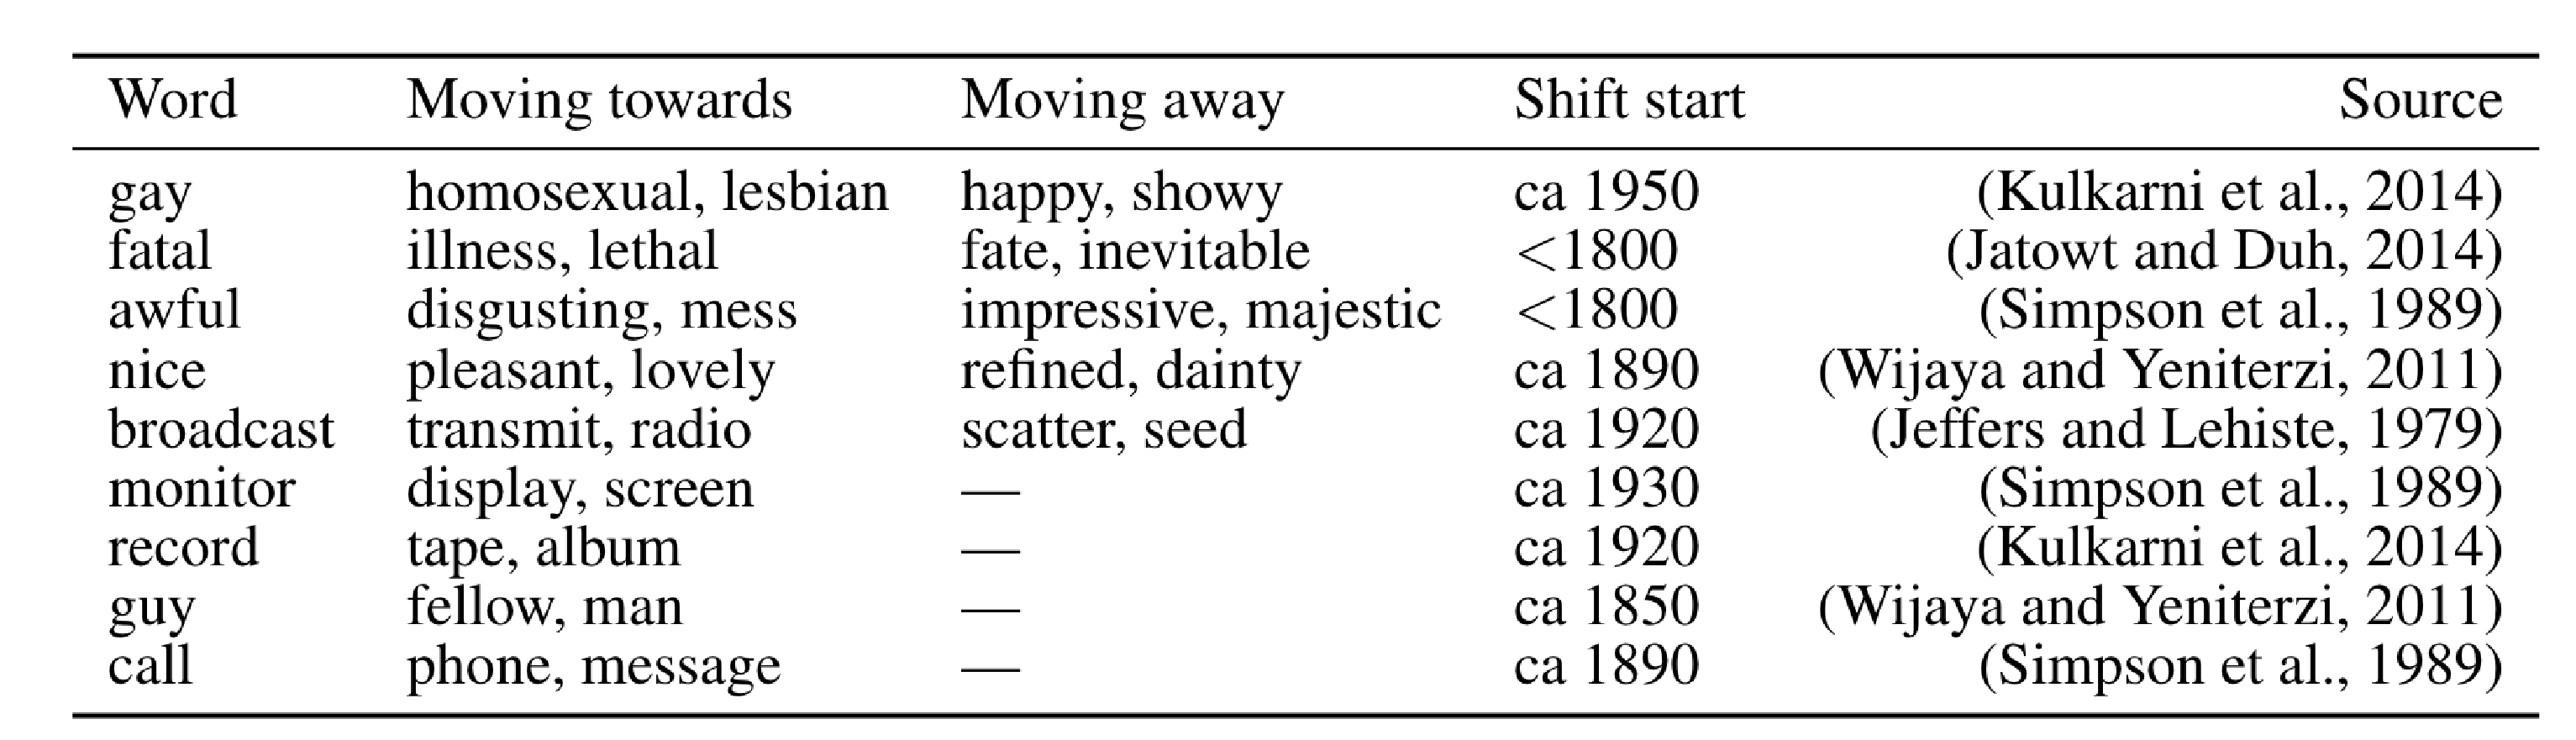
\includegraphics[scale=0.27]{figures/hamilton_known_shifts}
    \vspace*{-0.5cm}
    \caption{Known historical shifts from previous works (taken from \cite{hamilton-etal-2016-diachronic}).}
    \label{fig:hamilton-known-shifts}
\end{figure}

\textbf{Detecting Known Shifts:}
This task involves testing whether the methods can accurately capture historical shifts in word meanings that are already documented.
The goal is to determine if the methods can identify whether pairs of words have moved closer or further apart in semantic space over a specified time period.
The authors used a set of attested historical shifts as an evaluation set (\Cref{fig:hamilton-known-shifts}) to validate how well the embeddings capture these known changes.
These examples are taken from previous works on semantic change.

The results showed that all methods performed well in capturing the correct directionality of shifts, meaning they accurately identified whether word pairs became more similar or dissimilar over time.

\para{Discovering Shifts from data.}
In this task, the authors aimed to see if the methods could discover reasonable shifts in word meanings without prior knowledge of those shifts.
They examined the top-10 words that changed the most from the 1900s to the 1990s (\Cref{tab:discovering-shifts-table}) based on semantic displacement metric (\Cref{subsec:measuring-semantic-change}).
These words were categorized as \emph{genuine, borderline, or artifacts of the corpus} by the authors.

SGNS outperformed the other methods, with 70\% of its top-10 list corresponding to genuine semantic shifts, while SVD and PPMI had lower rates of genuine shifts.

\begin{table}[tbh]
\centering
\small
\begin{tabular}{@{}llll@{}}
\toprule
\rowcolor[HTML]{FFFFFF}
\multicolumn{1}{c}{\cellcolor[HTML]{FFFFFF}}                                          & \multicolumn{3}{c}{\cellcolor[HTML]{FFFFFF}\textbf{Examples}}                                                                                                                                                                                                                               \\ \cmidrule(l){2-4}
\rowcolor[HTML]{FFFFFF}
\multicolumn{1}{c}{\multirow{-2}{*}{\cellcolor[HTML]{FFFFFF}\textbf{Semantic Shift}}} & \multicolumn{1}{c}{\cellcolor[HTML]{FFFFFF}\textbf{PPMI}}                                                    & \multicolumn{1}{c}{\cellcolor[HTML]{FFFFFF}\textbf{SVD}}                  & \multicolumn{1}{c}{\cellcolor[HTML]{FFFFFF}\textbf{SGNS}}                                        \\ \midrule
\rowcolor[HTML]{EFEFEF}
\textbf{Genuine Shift}                                                                & started                                                                                                      & \begin{tabular}[c]{@{}l@{}}headed, calls,\\ gay, actually\end{tabular}    & \begin{tabular}[c]{@{}l@{}}wanting, gay, check, starting,\\ major, actually, headed\end{tabular} \\
\cellcolor[HTML]{FFFFFF}\textbf{Borderline}                                           & \begin{tabular}[c]{@{}l@{}}know, got, would, \\ decided, think, stop, \\ remember, must, wanted\end{tabular} & male, naturally                                                           & touching                                                                                         \\
\rowcolor[HTML]{EFEFEF}
\textbf{Corpus Artifact}                                                              & -                                                                                                             & \begin{tabular}[c]{@{}l@{}}harry, wherever,\\ special, cover\end{tabular} & harry, romance                                                                                   \\ \bottomrule
\end{tabular}
\caption{The top 10 words identified by each embedding method were examined, and after reviewing the literature and analyzing their nearest neighbors,
the authors categorized these words into different types of semantic shifts.
For instance, the word “headed” shifted from primarily meaning the “top of a body or entity” to signifying “a direction of travel” indicated a \emph{genuine} shift.
Additionally, some \emph{borderline} cases were identified, which were largely attributed to global shifts in genre or discourse, as well as corpus artifacts.
For example, words like “special,” “cover,” and “romance” appeared to be \emph{artifacts} from the covers of fiction books, occasionally influenced by advertisements,
taken from \cite{hamilton-etal-2016-diachronic}.}
\label{tab:discovering-shifts-table}
\end{table}


\subsection{Statistical Laws of Semantic Change}\label{subsec:statistical-laws-of-semantic-change}
The authors utilized diachronic embeddings to perform a large-scale cross-linguistic analysis,
revealing statistical laws that connect word frequency and polysemy to the rate of semantic change.

The authors quantified semantic change using the cosine distance metric between word embeddings across consecutive time periods, expressed as:
\begin{equation}
\Delta^{(t)}(w_i) = \text{cos-dist}(\mathbf{w}_i^{(t)}, \mathbf{w}_i^{(t+1)})
\label{eq:equation4}
\end{equation}

This equation measures how much a word’s meaning has shifted between two time periods t and t+1.
The value $\Delta^{(t)}(w_i)$ indicates the rate of semantic change for the word $w_i$.

To investigate the relationship between word frequency, polysemy, and semantic displacement, the authors performed regression analysis.
They considered data points for each word across pairs of consecutive decades.
Specifically, they analyzed how a word’s frequency and polysemy at time t correlated with its semantic displacement in the subsequent decade.

The analysis was restricted to non-stop words that appeared more than 500 times in both decades contributing to a change.
This criterion ensured that only words with sufficient co-occurrence data across years were included.

The authors employed a linear mixed model with random intercepts per word and fixed effects for frequency, polysemy, and per decade.
This model allowed them to estimate the effects of frequency and polysemy on semantic change while controlling for temporal trends and correcting for correlations between measurements on the same word across time.

\para{Law of conformity:} \emph{Frequently used words change at slower rates.}\\
The Law of Conformity states that the rates of semantic change scale with a negative power of word frequency.
This means that words that are used more frequently tend to change their meanings at a slower rate compared to less frequently used words.

This finding suggests that words with higher frequencies are more resistant to semantic shifts, confirming the Law of Conformity.
The authors demonstrated this law by presenting results using SGNS embeddings.

\para{Law of innovation:} \emph{Polysemous words change at faster rates.}\\
The Law of Innovation posits that words with higher levels of polysemy—meaning they have multiple meanings—experience higher rates of semantic change.
The authors measured a word’s polysemy by examining its neighborhood in an empirical co-occurrence network.
They constructed these networks for the top 10,000 non-stop words in each language using the Positive Pointwise Mutual Information (PPMI) measure.
In these networks, words are connected if they co-occur more often than would be expected by chance.
The polysemy of a word is then quantified by its local clustering coefficient within this network.
The clustering coefficient  $d(w_i)$  measures the proportion of a word  $w_i$’s neighbors that are also neighbors of each other.

A high clustering coefficient (and thus a low polysemy score) indicates that the words a given word co-occurs with also tend to co-occur with each other.
Conversely, polysemous words that appear in disjoint or unrelated contexts will have low clustering coefficients.

The authors found that the logarithm of the polysemy score exhibits a strong positive effect on rates of semantic change.
This finding supports the Law of Innovation by showing that words with more meanings (higher polysemy) change their meanings more rapidly.

\subsection{Takeaways}\label{subsec:takeaways4}
This paper explores how different types of word embedding models, such as PPMI, SVD, and SGNS, can be used to study diachronic shifts in word meanings.
By analyzing these aligned embeddings, the authors identify two key statistical laws of semantic change.
Law of conformity shows that high-frequency words have smaller semantic displacements over time.
They used statistical models to assess the relationship between word frequency and the rate of semantic change.
Specifically, they found that the logarithm of a word's frequency had a significant negative effect on the rates of semantic change, indicating that higher frequency words change less rapidly
The Law of Innovation is established by demonstrating that polysemous words—those with diverse meanings—tend to experience greater semantic change.
The clustering coefficient was used as a key metric for measuring polysemy within co-occurrence networks, revealing that words with lower clustering coefficients (higher polysemy) are more prone to semantic shifts.
This law highlights the dynamic nature of words with multiple meanings and their tendency to innovate in linguistic evolution.

